\setchapterpreamble[u]{\margintoc}
\chapter{Conclusions}
\labch{conclusions}
\label{sec:conclusions}

In this dissertation, we have proposed several methodologies for fusing information collected by multiple imaging sensors. The Enhanced Correlation Coefficient (\acrshort{ecc}), as proposed by Evangelidis and Psarakis \cite{evangelidis_parametric_2008}, is the baseline image matching algorithm that will help to compose a multi-layer system. It had not been yet explored for the alignment of heterogeneous datasets in Remote Sensing, albeit suiting particularly well images that have radiometric differences. It was demonstrated that the collected datasets depicting visible, infrared and multispectral wavelengths were accurately fused with an improved correlation coefficient. From here, this multi-layer system is translated to 3D point clouds which are easier to inspect by human operators. However, photogrammetry has already been proven to present geometrical inaccuracies over some kinds of imagery, including thermal and multispectral. Additionally, these have a lower resolution that inevitably leads to sparser point clouds. These drawbacks were tackled by estimating a baseline point cloud from high-resolution \acrshort{rgb} datasets, whereas the rest of the aligned information can be projected back to the point cloud. Hence, the multi-layer system was extended to 3D. Although hypercubes were not addressed before, this can also be projected to an \acrshort{rgb} point cloud. A different pipeline was followed according to the \textit{nadir} view angle, and therefore, the results were represented in 2.5D as a heightfield. These products, either in 2D or 3D, helped to support the following applications. Thermal imagery and point clouds were used in the identification of buried remains in an archaeological site. Then, hyperspectral swaths were processed and split into patches for the classification of grapevine varieties using Deep Learning.

Furthermore, some of the main disadvantages of real-world datasets are tackled by emulating how real sensors behave to generate synthetic datasets which can be augmented with any kind of information. Emulating imaging sensors is feasible, mainly with the rising importance of Generative Adversarial Networks, though we have narrowed these simulations to sensors which were not available. Hence, \acrshort{lidar} was simulated to generate large \acrshort{lidar} datasets that were proven to rapidly generate the outcome of large aerial and terrestrial surveys. This was further augmented with radiometric information; a comparison of two different techniques on the computation of intensity was checked. From the results, both approaches were able to produce point clouds with very notable differences among distinct surfaces. It was later applied to the optimization of \acrshort{lidar} scans using metaheuristics that helped to both reduce the number of scan positions and to optimize them.

On a technical level, these last three years have considerably contributed to improving as a researcher. The work carried out has led to important results that have been published in top journals and conferences from the Remote Sensing field, while others are still under review. In addition, I have had the pleasure of contributing to other colleagues' work, and despite those publications not fitting in this dissertation, they have greatly contributed to broadening my knowledge of Computer Graphics in other fields which are not my main area of expertise. 

\section{Summary of contributions}

In the first part of this dissertation, we explained a methodology for correcting and fusing images from multiple data sources at the image level. The Enhanced Correlation Coefficient was proposed as a technique fitting the requirements of remotely sensed images focused on different wavelength intervals. It behaved surprisingly well over datasets with significant radiometric differences. This method was massively applied to match visible, multispectral and infrared datasets. Furthermore, this image-matching algorithm was checked to highlight how efficient is it, since it provides remarkable results even for lower image dimensions and distortions, such as noise. In fact, partly missing some of the details helped in reducing significantly the response time.

This image-matching procedure denotes the baseline of this dissertation as well as of the following part. It has already been remarked the advantages, and disadvantages, of working with images or point clouds. Hence, the latter is better for some specific applications as they enable visualizing one area at a glance, whereas location awareness is considerably improved for tasks performed by human operators. However, these are not as helpful if point clouds are sparse or present geometrical inaccuracies. Therefore, we presented a formal framework for the generation of point clouds comprising visible, thermal and multispectral point clouds. A dense and large visible point cloud was first achieved using photogrammetry, but the rest of the datasets were projected into this accurate and dense point cloud. It tackles the most frequent drawbacks of photogrammetry along with thermal and multispectral imagery. It was also shown to outperform commercial software in terms of 1) response time, 2) density and 3) size. Projection, on the other hand, must be aware of occlusion to achieve colourimetrically accurate results. This was handled using two methods; firstly, occlusion is taken into account with a traditional depth buffer, whereas the aggregation of remaining image samples in every 3D point was achieved using aggregation and penalty functions. The latter helps to compute an aggregated colour that minimizes the distance from a collection of samples. 

Besides projection and occlusion-aware considerations, this pipeline was implemented in the \acrshort{gpu}, similar to commercial software such as Agisoft Metashape or Pix4Dmapper. Yet, our methodology outperformed these commercial solutions in terms of response time. Other enhancements were tested, as proposed by Schutz et al. \cite{schutz_rendering_2021}, where the reordering of the point cloud was performed either globally or in small groups. The tests carried out showed that globally reordering the point cloud significantly improved the response time, despite adding the latency derived from sorting. On the other hand, shuffling these sorted point clouds using small groups did not achieve better results as the sorting + shuffling overhead worsens the results of processes that are solely launched once.  

The second part also comprises the generation of hyperspectral point clouds, which to the best of our knowledge, had not been achieved previously, at least in nature. It required stitching the hyperspectral swaths and an RGB orthomosaic to compose a hyperspectral orthomosaic. This was later projected onto the voxelization of a 3D point cloud, also known as heightfields. This led to generating 2.5D products rather than 3D since hyperspectral datasets were collected with \textit{nadir} view direction. The \acrshort{gsd} was adapted to the resolution of this imagery, and despite occlusion not being a drawback here, samples from overlapping swaths were aggregated into the heightfields according to aggregation and penalty functions. Given the large size of the resulting hypercube, it was compressed in the radiometric dimension by following the approach of Graciano et al. \cite{graciano_real-time_2018}. The majority of steps were implemented in the \acrshort{gpu}, and besides that, the aftermath of compressing the spectral heightfields was a data structure that was slightly harder to traverse in real-time. Hence, this drawback was alleviated by composing images in multiple frames. Similar to previous work, the point cloud visualization was enhanced using OpenGL's compute shaders, taking advantage of modern extensions.

Once this core was defined, the multi-layer system still lacked other widespread sensor products, such as \acrshort{lidar}. It was simulated through the Time of Flight principle plus systematic and random errors described in the literature. Atmospheric particles, highly reflective surfaces or slope- and height-derived errors were included, whereas the synthetic sensor was parameterized so that it can be fed with the specifications of nowadays commercial sensors. Furthermore, previous work had already solved part of this and proposed to emulate \acrshort{lidar} to generate \acrshort{lidar} datasets for Deep Learning. However, another key factor is the synthetic scenarios which are later scanned; in this work, these were procedurally generated to compute a large number of point clouds. The scenarios are first labelled and linked to materials according to name patterns, which facilitates this manual task. For procedural scenes, this task is only performed once to build environments with varying distributions that follow some pre-defined rules. Nonetheless, static scenes were also included and can be labelled as explained. Finally, a comparison was established on the calculation of return intensity; first, it was modelled using traditional Computer Graphics \acrshort{brdf}s, and then, these were simulated using real-world measurements as obtained from a goniophotometer. The comparison with real-world point clouds is hard to establish, and therefore, the experiments were carried out by showing the histograms of scenarios with different materials. This simulation was entirely wrapped in the \acrshort{gpu} to supply rapid aerial and terrestrial surveys, from the generation of \acrshort{lidar} beams to scanning.

Unlike previous \acrshort{lidar} simulators, ours was also intended to simulate terrestrial and airborne surveys. The first is the most common, whereas the latter has been barely addressed. Both are articulated over the interpolation of temporal locations from a path, either user-defined or automatically computed. However, airborne surveys also require the simulation of different scanning patterns, from which parallel, zigzag and elliptical patterns were included. In airborne missions, multiple returns are especially relevant since they allow filtering out canopy and vegetation, whereas bathymetry helps to survey shallow underwater areas. 

Datasets and results from previous chapters were utilized in practical case studies. Firstly, hyperspectral swaths were corrected and applied to the classification of seventeen grapevine varieties, either belonging to red or white variants. Traditional techniques, based on the correlation of spectral signatures, do not fit case studies where the signatures' shapes are very similar. Instead, a Deep Learning network was explored for the classification of grapevine varieties, using state-of-the-art blocks, such as Inception or spatial attention. Hypercubes were split into patches, whose size was tuned during experimentation, and they were reduced to a single label; hence, the classification of every sample was influenced by its neighbourhood. Not only this network was proven to perform well over \acrshort{uas} datasets, but they also were able to obtain results close to the the-start-of-the-art overall accuracy. Then, thermal imagery and point clouds were applied to inspecting an archaeological site, where two anomalous areas were spotted in areas that may correspond to the location of buried towers. 

\section{Future work}

Remote sensing and Deep Learning fields are rapidly evolving, and yet, there exist some future investigations that should be explored from this work:
\begin{itemize}
    \item Image matching was performed using commodity hardware, and therefore, it was explored whether downscaling and blur led to better response time. Indeed, it offered similar results with lower latency. From here, it could be explored if a pyramid scheme, from lower to higher size, helps to obtain better results while yet obtaining a low latency. This way, larger transformations are computed from low-resolution imagery, whereas the most fine-grained changes are calculated with the starting dimensions. Besides reducing the response time, this approach could also help to match images with more notable differences.
    \item Image-matching was included as part of the reading phase in the comparisons established with commercial photogrammetry software. Therefore, this stage can be further accelerated by transferring the \acrshort{ecc} algorithm, currently obtained from OpenCV, to the \acrshort{gpu}.
    \item The generation of dense and large visible, thermal and multispectral point clouds helps to better visualize the scenario; however, point clouds with such a dimensionality are also harder to render in real-time. Although the compute-shader rendering alleviated this drawback \cite{schutz_rendering_2021}, it could be further enhanced with different levels of detail (\acrshort{lod}) \cite{schutz_gpu-accelerated_2023}. Similarly, it could help in the rendering of compressed hypercubes, since we already had to expand its real-time rendering over a few frames until completion.
    \item The compression of hypercubes was achieved by lowering the radiometric resolution with a stack-based representation, whereas spatial compression was not possible since surrounding stacks were very different. Rather than a stack-based representation, compression could be achieved in the spatial dimension, which is known to be way larger than the spectral one. 
    \item \acrshort{lidar} optimization was studied as the simplest case study: a set of optimal locations that help to survey a scene with \acrshort{tls}. However, there are other kinds of \acrshort{lidar} which may be worth exploring, such as those that rely on a path rather than a set of locations. Swarm-based optimizations may fit better if a path is required \cite{roberge_fast_2018}. Optimization of airborne \acrshort{lidar} could also be explored to determine which is the optimal configuration to densely scan a scene from a DSM, including, but not limited to the followed path.
    \item A similar approach to the latter proposal is to assess \acrshort{uas} missions by computing a path that guarantees the required overlap or coverage according to the time, altitude and \acrshort{uas} flight speed, among other factors. This has been achieved for generic \acrshort{uas} missions \cite{pessacg_simplifying_2022}, though it could be further improved based on the scene geometry, represented by rapidly sketched models. It could be especially relevant for oblique view directions, by setting it as an optimizable parameter rather than a user-defined factor. 
    \item So far, the \acrshort{lidar} simulations have helped to generate large \acrshort{lidar} datasets. However, there still remain some experiments that ought to be carried out to check whether these datasets are helpful for Deep Learning tasks. Note that some of the simulated errors will be filtered out once the point clouds are voxelized, which is the most widespread approach for feeding \acrshort{lidar} datasets \cite{hackel_semantic3d_2017, behley_towards_2021}. However, it should be discerned if these synthetic datasets are similar enough to the point distribution generated by real sensors. 
    \item Part IV only explained the simulation of \acrshort{lidar} sensors, which were unavailable at that time. However, other sensors can be simulated by means of synthetically generated imagery. Generative Adversarial Networks (\acrshort{gan}) have been gaining interest as they allow building computer-made unsupervised datasets, from art to simple texts. Besides \acrshort{lidar}, infrared data could be simulated from visible imagery to create larger datasets. The current state-of-the-art has not successfully achieved this task by learning solely from visible data \cite{li_multi-branch_2019, li_i-gans_2021, kniaz_thermalgan_2019, ozkanoglu_infragan_2022, yi_cycle_2023}, since it may require semantic annotations to isolate surfaces that have different radiance. 
    \item The phenotyping of grapevine varieties was approached with Deep Learning; however, this model could be improved by further integrating more varieties and collecting datasets at different stages of the year. Also, there are other interesting approaches to address this very same task, from multi-instance \cite{meerdink_multitarget_2022} to contrastive learning \cite{guan_spatial-spectral_2022}. 
\end{itemize}

\begin{figure}
    \centering
    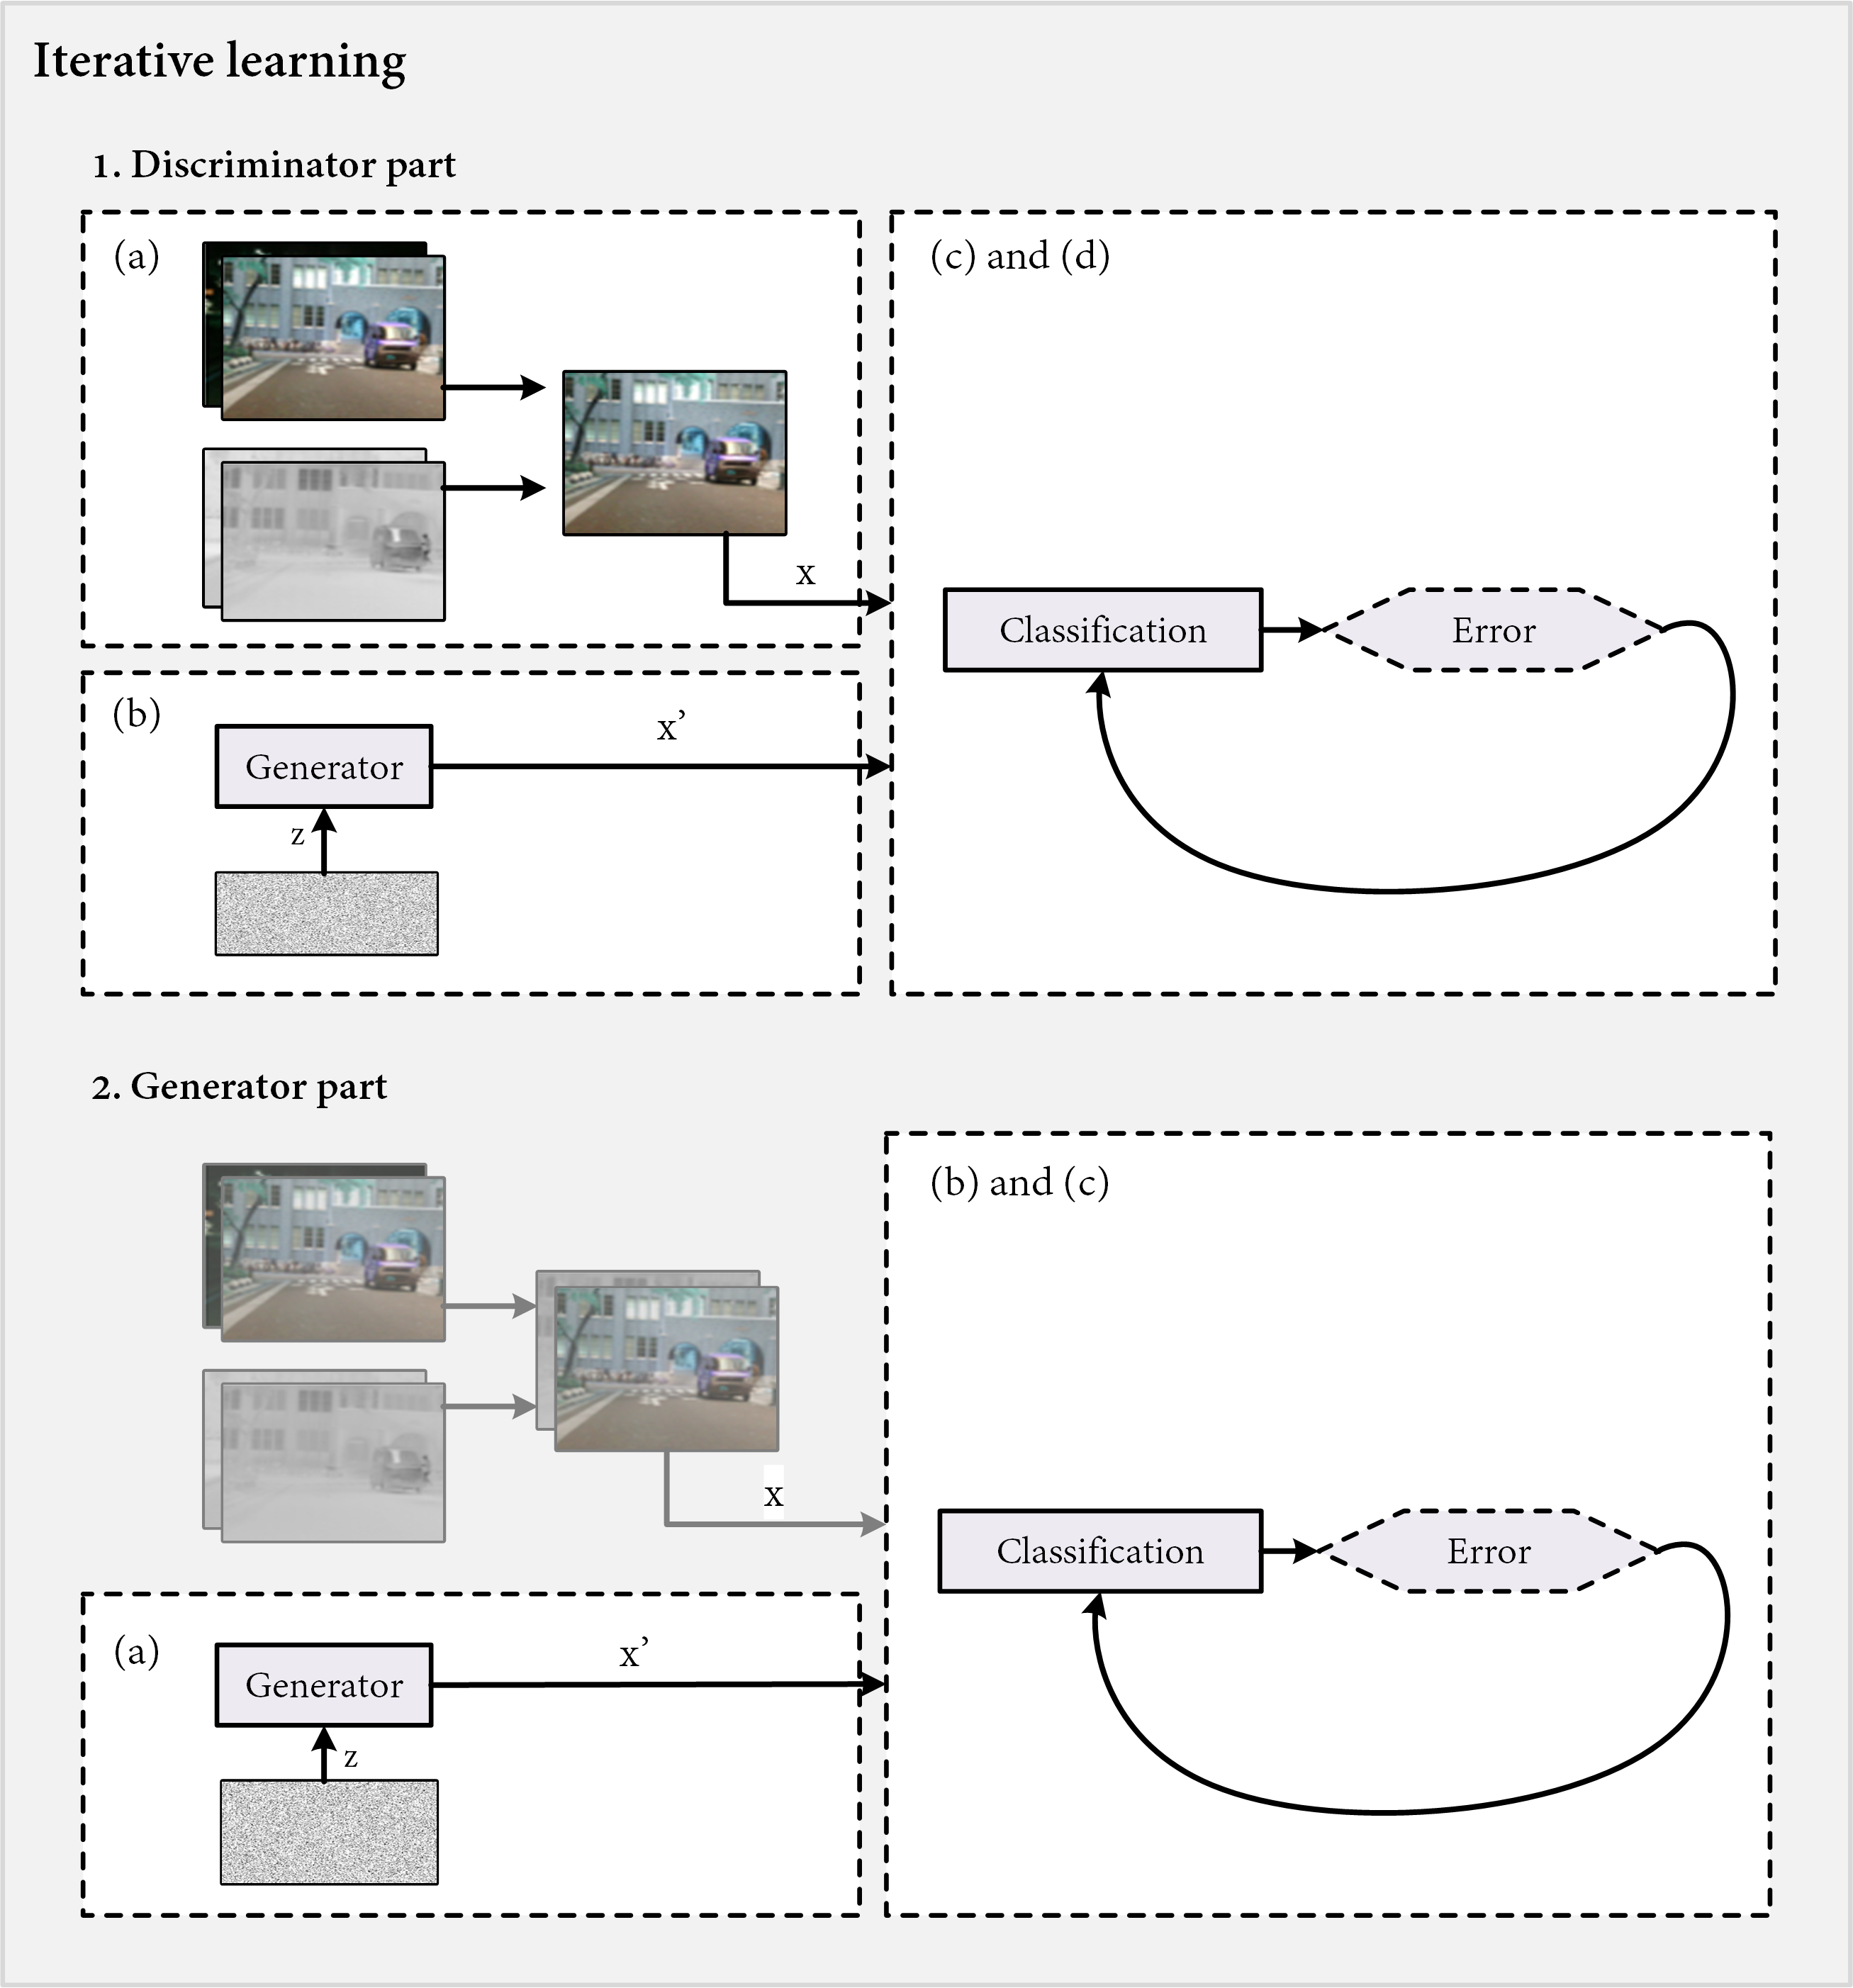
\includegraphics[width=\linewidth]{figs/conclusions/gan.png}
    \caption{Overview of the proposed \acrshort{lidar} simulation. First, scenes are modelled either as static or procedural, linked to semantic labels as well as to materials properties. Then, a virtual \acrshort{lidar} iteratively solves the simulation and its result is stored in a standard file format.}
    \label{fig:conclusions_gan}
\end{figure}